  \begin{figure}[ht]
    \centering
    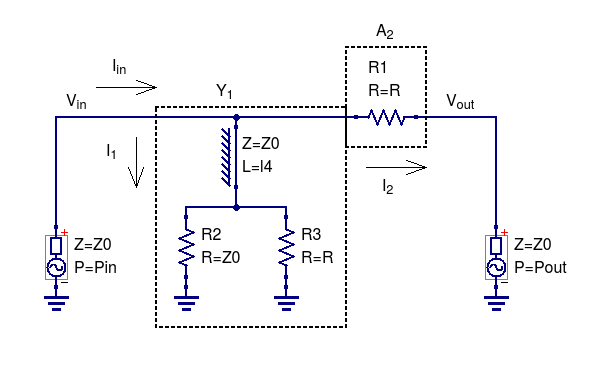
\includegraphics[width=10cm]{./images/qw-shunt-attenuator-schematic.png}
    \caption{Quarter wavelength shunt attenuator}
    \label{fig:qw-shunt-attenuator-schematic}
  \end{figure}
  
\noindent At the center frequency, the $\lambda/4$ transmission line behaves as an impedance inverter and its input impedance is given by:

\begin{equation}
	Z_{TL} = \frac{Z_0^2}{Z_L}, Z_L = \frac{R \cdot Z_0}{R + Z_0} \Rightarrow Z_{TL} = Z_0 \cdot \frac{R + Z_0}{R}
\end{equation}

\noindent The ABCD parameters of the shunt branch ($Y_2$) are the following:

\begin{equation}
	Y_1 = \begin{pmatrix}
				1 & 0\\
				\frac{R}{Z_0 \cdot (R+Z_0)}  & 1
		\end{pmatrix}
\end{equation}

\noindent The ABCD parameters of the series resistor is:
\begin{equation}
	A_2 = \begin{pmatrix}
				1 & R\\
				0  & 1
		\end{pmatrix}
\end{equation}

\noindent Therefore, the ABCD parameters of the whole quarter-wavelength attenuator is simply the product of $Y_1$ and $A_2$:

\begin{equation}
	A_{qw_{shunt}} = Y_1 \cdot A_1 = \begin{pmatrix}
											1 & R\\
											\frac{R}{Z_0 \cdot(R+Z_0)}  & 1 + \frac{R^2}{Z_0 \cdot(R+Z_0)}
									\end{pmatrix}
\end{equation}

\noindent Using the conversion formulae between ABCD and S parameters \cite{pozar2012microwave}:
\begin{equation}
	S_{qw_{shunt}} = \begin{pmatrix}
							0 & \frac{Z_0}{R + Z_0}\\
							\frac{Z_0}{R+Z_0}  & \frac{R^2}{(R+Z_0)^2}
					 \end{pmatrix}
\end{equation}

\noindent and the attenuation (in dB) is obtained in terms of R and $Z_0$ as:

\begin{equation}
	\alpha = -20 \cdot log_{10} \left( \frac{Z_0}{R + Z_0}\right)
\end{equation}

\noindent Thus, the resistor value is determined by the attenuation and the system impedance as:

\begin{equation}
 	R = Z_0 \cdot \left( 10^{\frac{\alpha}{20}} - 1 \right)
\end{equation}

\noindent and the output impedance is:

\begin{equation}
	Z_{out} = R + Z_1 \parallel Z_0 = R + \frac{Z_0 \cdot (R + Z_0)}{2 \cdot R + Z_0}
\end{equation}

\noindent Concerning power dissipation, the power dissipated in the shunt branch is:

\begin{equation}
	P_{shunt} = \frac{V_{in}^2}{Z_{TL}} = P_{in} \cdot \frac{R}{R+Z_0}
\end{equation}

\noindent The voltage at the node between the transmission line and the shunt resistors may be expressed as:

\begin{equation}
	V_{1} = \sqrt{P_{shunt} \cdot R_{eq}} = R \cdot \frac{\sqrt{P_{in} \cdot Z_0}}{R + Z_0}
\end{equation}

\noindent Thus, the power dissipated in $R_2$ and $R_3$ is given by:

\begin{equation}
	P_{R2} = P_{in} \cdot \frac{R^2}{(R + Z_0)^2}
\end{equation}

\begin{equation}
	P_{R3} = P_{in} \cdot \frac{R \cdot Z_0}{(R + Z_0)^2}
\end{equation}

\noindent Being $I_1 = \frac{V_{in}}{Z_{TL}}$ the current flowing through the shunt branch and $I_{in} = \sqrt{\frac{P_{in}}{Z_{TL}}}$ the current delivered by the source, the current through $R_1$ and the load is $I_2 = I_{in} - I_1$ and, consequently, the power dissipated in $R_1$ is:

\begin{equation}
	P_{R1} = P_{in} \cdot \frac {R \cdot Z_0}{(R+Z_0)^2}
\end{equation}